% das Papierformat zuerst
\documentclass[a4paper, 11pt]{article}
\usepackage[margin=3cm]{geometry}
\usepackage[utf8]{inputenc}
\usepackage[T1]{fontenc}
\usepackage{hyperref} % clickable refs
\usepackage{graphicx}
\usepackage[toc, numberedsection]{glossaries}
\usepackage{float}
\usepackage{amssymb}

% TODO: template übersetzten

\makeglossaries

%Hack for referencing labels
\makeatletter
\def\namedlabel#1#2{\begingroup
    #2%
    \def\@currentlabel{#2}%
    \phantomsection\label{#1}\endgroup
}
\makeatother
% End: Hack for referencing labels

% Glossar: alle Einträge, aber ohne extra Referenzen
% http://tex.stackexchange.com/questions/115635/glossaries-suppress-pages-when-using-glsaddall
\newcommand*{\glsgobblenumber}[1]{}
\makeatletter
\newcommand*{\glsaddnp}[2][]{
  \glsdoifexists{#2}{
    \def\@glsnumberformat{glsgobblenumber}
    \edef\@gls@counter{\csname glo@#2@counter\endcsname}
    \setkeys{glossadd}{#1}
    \@gls@saveentrycounter
    \@do@wrglossary{#2}
  }
}
\renewcommand{\glsaddallunused}[1][]{
  \edef\@glo@type{\@glo@types}
  \setkeys{glossadd}{#1}
  \forallglsentries[\@glo@type]{\@glo@entry}{
    \ifglsused{\@glo@entry}{}{
      \glsaddnp[#1]{\@glo@entry}}}
}
\makeatother

\renewcommand{\glsnamefont}[1]{\mdseries #1} % glossary entries shouldn’t be bold

% Glossar

% So sieht ein Glossar-Eintrag aus:
%
%\newglossaryentry{dijkstra}{
%  name={Dijkstra’s Algorithmus},
%  description={ein Algorithmus, um den optimalen Pfad in einem gerichteten Graphen zu finden}
%}
%\newglossaryentry{arc}{
%  name={Arc-Flags},
%  description={eine Technik, um Routenberechnung zu beschleunigen},
%  see={dijkstra}
%}
%
% Und so kann er im Dokument verwendet werden:
%
% lorem ipsum dolor sit \gls{arc}, consectetur
%
% End: Glossar

% usage: \counteditem{prefix}{refName} -> item `/prefixXX/` with label `prefix:refName` (where XX is counted in increments of 10)
\makeatletter
\newcommand{\oitem}[2]{
  % define the counter
  \@ifundefined{c@oitem#1}{\newcounter{oitem#1}}{} % initialized at 0
  \addtocounter{oitem#1}{10}
  \item[\namedlabel{#1:#2}{/#1\arabic{oitem#1}/}]
}
\makeatother

% usage: \testfall{szenario}{ablauf}{ergebnis} oder \testfall[\ref{F:getesteteFunktion}]{szenario}{ablauf}{ergebnis}
\newcommand{\testfall}[4][]{
  \begin{description}
    \ifthenelse{\equal{#1}{}}
               {} % optional argument #1 is empty: skip
               {\item[Testet] #1}
    \item[Vorbedingungen] #2
    \item[Ablauf] #3
    \item[Erwartetes Ergebnis] #4
  \end{description}
}

\begin{document}

% place a symbol before clickable links
% this has to come *after* \begin{document} because hyperref installs a \AtBeginDocument hook that updates the ref command.
\newcommand{\refsymbol}[0]{\scalebox{0.5}{$\nearrow$}}
\let\oldref\ref
\renewcommand{\ref}[1]{\refsymbol\oldref{#1}}
\let\oldgls\gls
\renewcommand{\gls}[1]{\refsymbol\oldgls{#1}}
\let\oldGls\Gls
\renewcommand{\Gls}[1]{\refsymbol\oldGls{#1}}
\let\oldglspl\glspl
\renewcommand{\glspl}[1]{\refsymbol\oldglspl{#1}}
\let\oldGlspl\Glspl
\renewcommand{\Glspl}[1]{\refsymbol\oldGlspl{#1}}
\let\oldglslink\glslink
\renewcommand{\glslink}[2]{\refsymbol\oldglslink{#1}{#2}}
\let\oldhyperref\hyperref
\renewcommand{\hyperref}[2][notActuallyOptional]{\refsymbol\oldhyperref[#1]{#2}}
\let\oldautoref\autoref
\renewcommand{\autoref}[1]{\refsymbol\oldautoref{#1}}

\newcommand{\abbildung}[1]{\autoref{fig:#1}}
\newcommand{\mamid}[0]{\textit{KIT-MAMID} }

% alle Glossareintraege
\newacronym{gui}{GUI}{Graphical User Interface}
\newacronym{cli}{CLI}{Command Line Interface}

\newglossaryentry{cluster}{
  name={cluster},
  description={It's something.},
  plural={clusters}
}
\newglossaryentry{MongoDB}{
	name={MongoDB},
	description={It's something.},
	plural={MongoDB}
}
\newglossaryentry{replica set}{
	name={replica set},
	description={It's something.},
	plural={replica sets}
}
\newglossaryentry{administrator}{
	name={administartor},
	description={It's something.},
	plural={administrators}
}
\newglossaryentry{host}{
	name={host},
	description={It's something.},
	plural={hosts}
}
\newglossaryentry{slave}{
	name={slave},
	description={It's something.},
	plural={slaves}
}
\newglossaryentry{master}{
	name={master},
	description={It's something.},
	plural={masters}
}
\newglossaryentry{inventory}{
	name={inventory},
	description={It's something.},
	plural={inventories}
}
\newglossaryentry{disabled mode}{
	name={disabled mode},
	description={It's something.},
	plural={}
}
\newglossaryentry{physical interdependency}{
	name={physical interdependency},
	description={It's something.},
	plural={physical interdependencies}
}
\newglossaryentry{maintenance mode}{
	name={maintence mode},
	description={It's something.},
	plural={}
}
\newglossaryentry{persistent storage}{
	name={persistent storage},
	description={It's something.},
	plural={}
}
\newglossaryentry{volatile storage}{
	name={volatile storage},
	description={It's something.},
	plural={}
}
\newglossaryentry{root data directory}{
	name={root data directory},
	description={It's something.},
	plural={hosts}
}
\newglossaryentry{arbiter}{
	name={arbiter},
	description={It's something.},
	plural={hosts}
}
\newglossaryentry{degraded}{
	name={degraded},
	description={It's something.},
	plural={hosts}
}
\newglossaryentry{HTTP API}{
	name={HTTP API},
	description={It's something.},
	plural={hosts}
}
\newglossaryentry{active mode}{
	name={active mode},
	description={It's something.},
	plural={hosts}
}
\begin{titlepage}
\makeatletter
\begin{center}
~\\[5em]
{\Huge KIT-MAMIT}\\[3em]
{\huge Functional specification}\\[1em]
{\large\today}\\[2.5em]
{\LARGE
Niklas Fuhrberg\\
Anton Schirg\\
Christian Schwarz\\
Janis Streib\\
Bob Weinand\\[3em]}
supervised by\\[2em]
{\Large
Dr. Marek Szuba\\[1em]}
at\\[1em]
{\Large
Karlsruhe Institute of Technology\\
SCC}

\end{center}
\makeatother
\end{titlepage}
\newpage
\tableofcontents
\newpage

% -------------------------------------------------------------- HIER BEGINNT DAS DOKUMENT WIRKLICH ---------------------------------
\section{Introduction}
\mamid is a manager for database \glspl{cluster}, facilitating creation, administration and monitoring of \gls{MongoDB} \glspl{replica set}.

\mamid assists the \gls{administrator} during initial setup, continuous operation, maintenance cases and expansion of the cluster.

Each cluster \gls{host} runs a \gls{slave} instance of \mamid.
A single \gls{master} instance coordinates the \glspl{slave}' membership in the \glspl{replica set}.

\section{Zielbestimmung}
\subsection{Musskriterien}

\begin{description}

\oitem{MK}{} The \gls{administrator} interacts with \mamid through a web \acrshort{gui}.

% inventory ops
\oitem{MK}{} The \gls{master} maintains a list of \glspl{slave} called \gls{inventory}.
\oitem{MK}{} The \gls{administrator} can add \glspl{slave} to the \gls{inventory}.
\oitem{MK}{} The \acrshort{gui} visualizes the \gls{inventory}.
\oitem{MK}{} The \gls{administrator} can remove a \gls{slave} in \gls{disabled mode} from the \gls{inventory}.
\oitem{MK}{} The \gls{administrator} can specify \glspl{physical interdependency} between \gls{inventory} \glspl{slave}.

% inventory ops -> slave
\oitem{MK}{} The \gls{administrator} can set set a \gls{slave} in the \gls{inventory} to one of the following modes: \gls{active mode}, \gls{maintenance mode}, \gls{disabled mode}.
\oitem{MK}{} The \gls{administrator} can set a \gls{slave} as either \glslink{persistent storage}{persistent} \glslink{volatile storage}{volatile}.
\oitem{MK}{} The \gls{administrator} can specify a \gls{root data directory} per \gls{slave}.

% replica set ops
\oitem{MK}{} The \gls{administrator} can create a new \gls{replica set}.
\oitem{MK}{replica_set_member_counts} The \gls{administrator} can select the counts $p,v \in $ of (\glslink{persistent storage}{\textbf{p}ersisent} / \glslink{volatile storage}{\textbf{v}olatile}) \gls{replica set} members, where $(p+v) > 2 \land p >= 1 \land (p+v) \text{ odd}$.
\oitem{MK}{} The \acrshort{gui} visualized the list of configured \glspl{replica set}.
\oitem{MK}{} The \gls{administrator} can destroy a \gls{replica set}.
\oitem{MK}{} The \gls{master} deploys the \gls{replica set} configuration to the cluster.

% slaves
\oitem{MK}{} The \gls{slave} controls \gls{MongoDB} processes on the \gls{cluster} \glspl{host}.

% monitoring features
\oitem{MK}{detect_slave_unexpected_behavior} The \gls{master} detects when a \gls{slave} in the \gls{inventory} behaves unexpectedly.
\oitem{MK}{} The \gls{master} informs the \gls{administrator} by e-mail about problems in the cluster (\ref{MK:detect_slave_unexpected_behavior}).
\oitem{MK}{} The \acrshort{gui} visualizes \glspl{slave} behaving unexpectedly (\ref{MK:detect_slave_unexpected_behavior}).

\end{description}

\subsection{Wunschkriterien}
\begin{description}
	
% inventory
\oitem{WK}{} The \gls{master} auto-discovers new \glspl{slave} on the \gls{administrator}'s request.
\oitem{WK}{} The \gls{master} continuously auto-discovers \glspl{slave}.
\oitem{WK}{} The \gls{master} monitors reachability of \gls{cluster} \glspl{host} via ICMP.

% slaves
\oitem{WK}{} The \gls{administrator} can specify arbitrary \gls{MongoDB} command line parameters per \gls{slave}.
\oitem{WK}{} The \gls{administrator} can specify a \gls{MongoDB} configuration file template.

% automatic repair
\oitem{WK}{} The \gls{master} automatically repairs \gls{degraded} \glspl{replica set} with \emph{suitable} \glslink{active mode}{active} \glspl{slave}.

% replica sets
\oitem{WK}{} The \gls{master} deploys \gls{MongoDB} \glspl{arbiter} for configured \glspl{replica set}, removing some restrictions in \ref{MK:replica_set_member_counts}.
\oitem{WK}{} The \gls{master} exposes machine metrics of the \glspl{slave}.
\oitem{WK}{} The \gls{master} exposes the \glspl{replica set}' replication status.

% other
\oitem{WK}{} The \gls{administrator} can interact with \mamid via a \acrshort{cli}.
\oitem{WK}{} The \gls{administrator} can interact with \mamid via a \gls{HTTP API}.
\end{description}

\subsection{Abgrenzungskriterien}
\begin{description}
\oitem{AK}{} The \gls{master} does not implement support for higher-layer \gls{MongoDB} features, e.g. \emph{Sharding}.
\oitem{AK}{} \mamid neither deploys the operating system nor other required software (such as \gls{MongoDB} binaries) to the \gls{cluster} \glspl{host}.
\end{description}

\section{Produkteinsatz}

\subsection{Anwendungsbereiche}
\begin{itemize}
\item foo
\end{itemize}

\subsection{Zielgruppe}
\begin{itemize}
\item foo
\end{itemize}

\subsection{Betriebsbedingungen}
\begin{itemize}
\item zu Hause (test)
\end{itemize}

\section{Produktumgebung}
%Kevin

\subsection{Software}\label{subsec:Software}

\begin{itemize}
\item Operating system: Solaris (Indiana OS), Linux
\end{itemize}

\subsection{Hardware}

\begin{itemize}
\item foo
\end{itemize}
\section{System model}
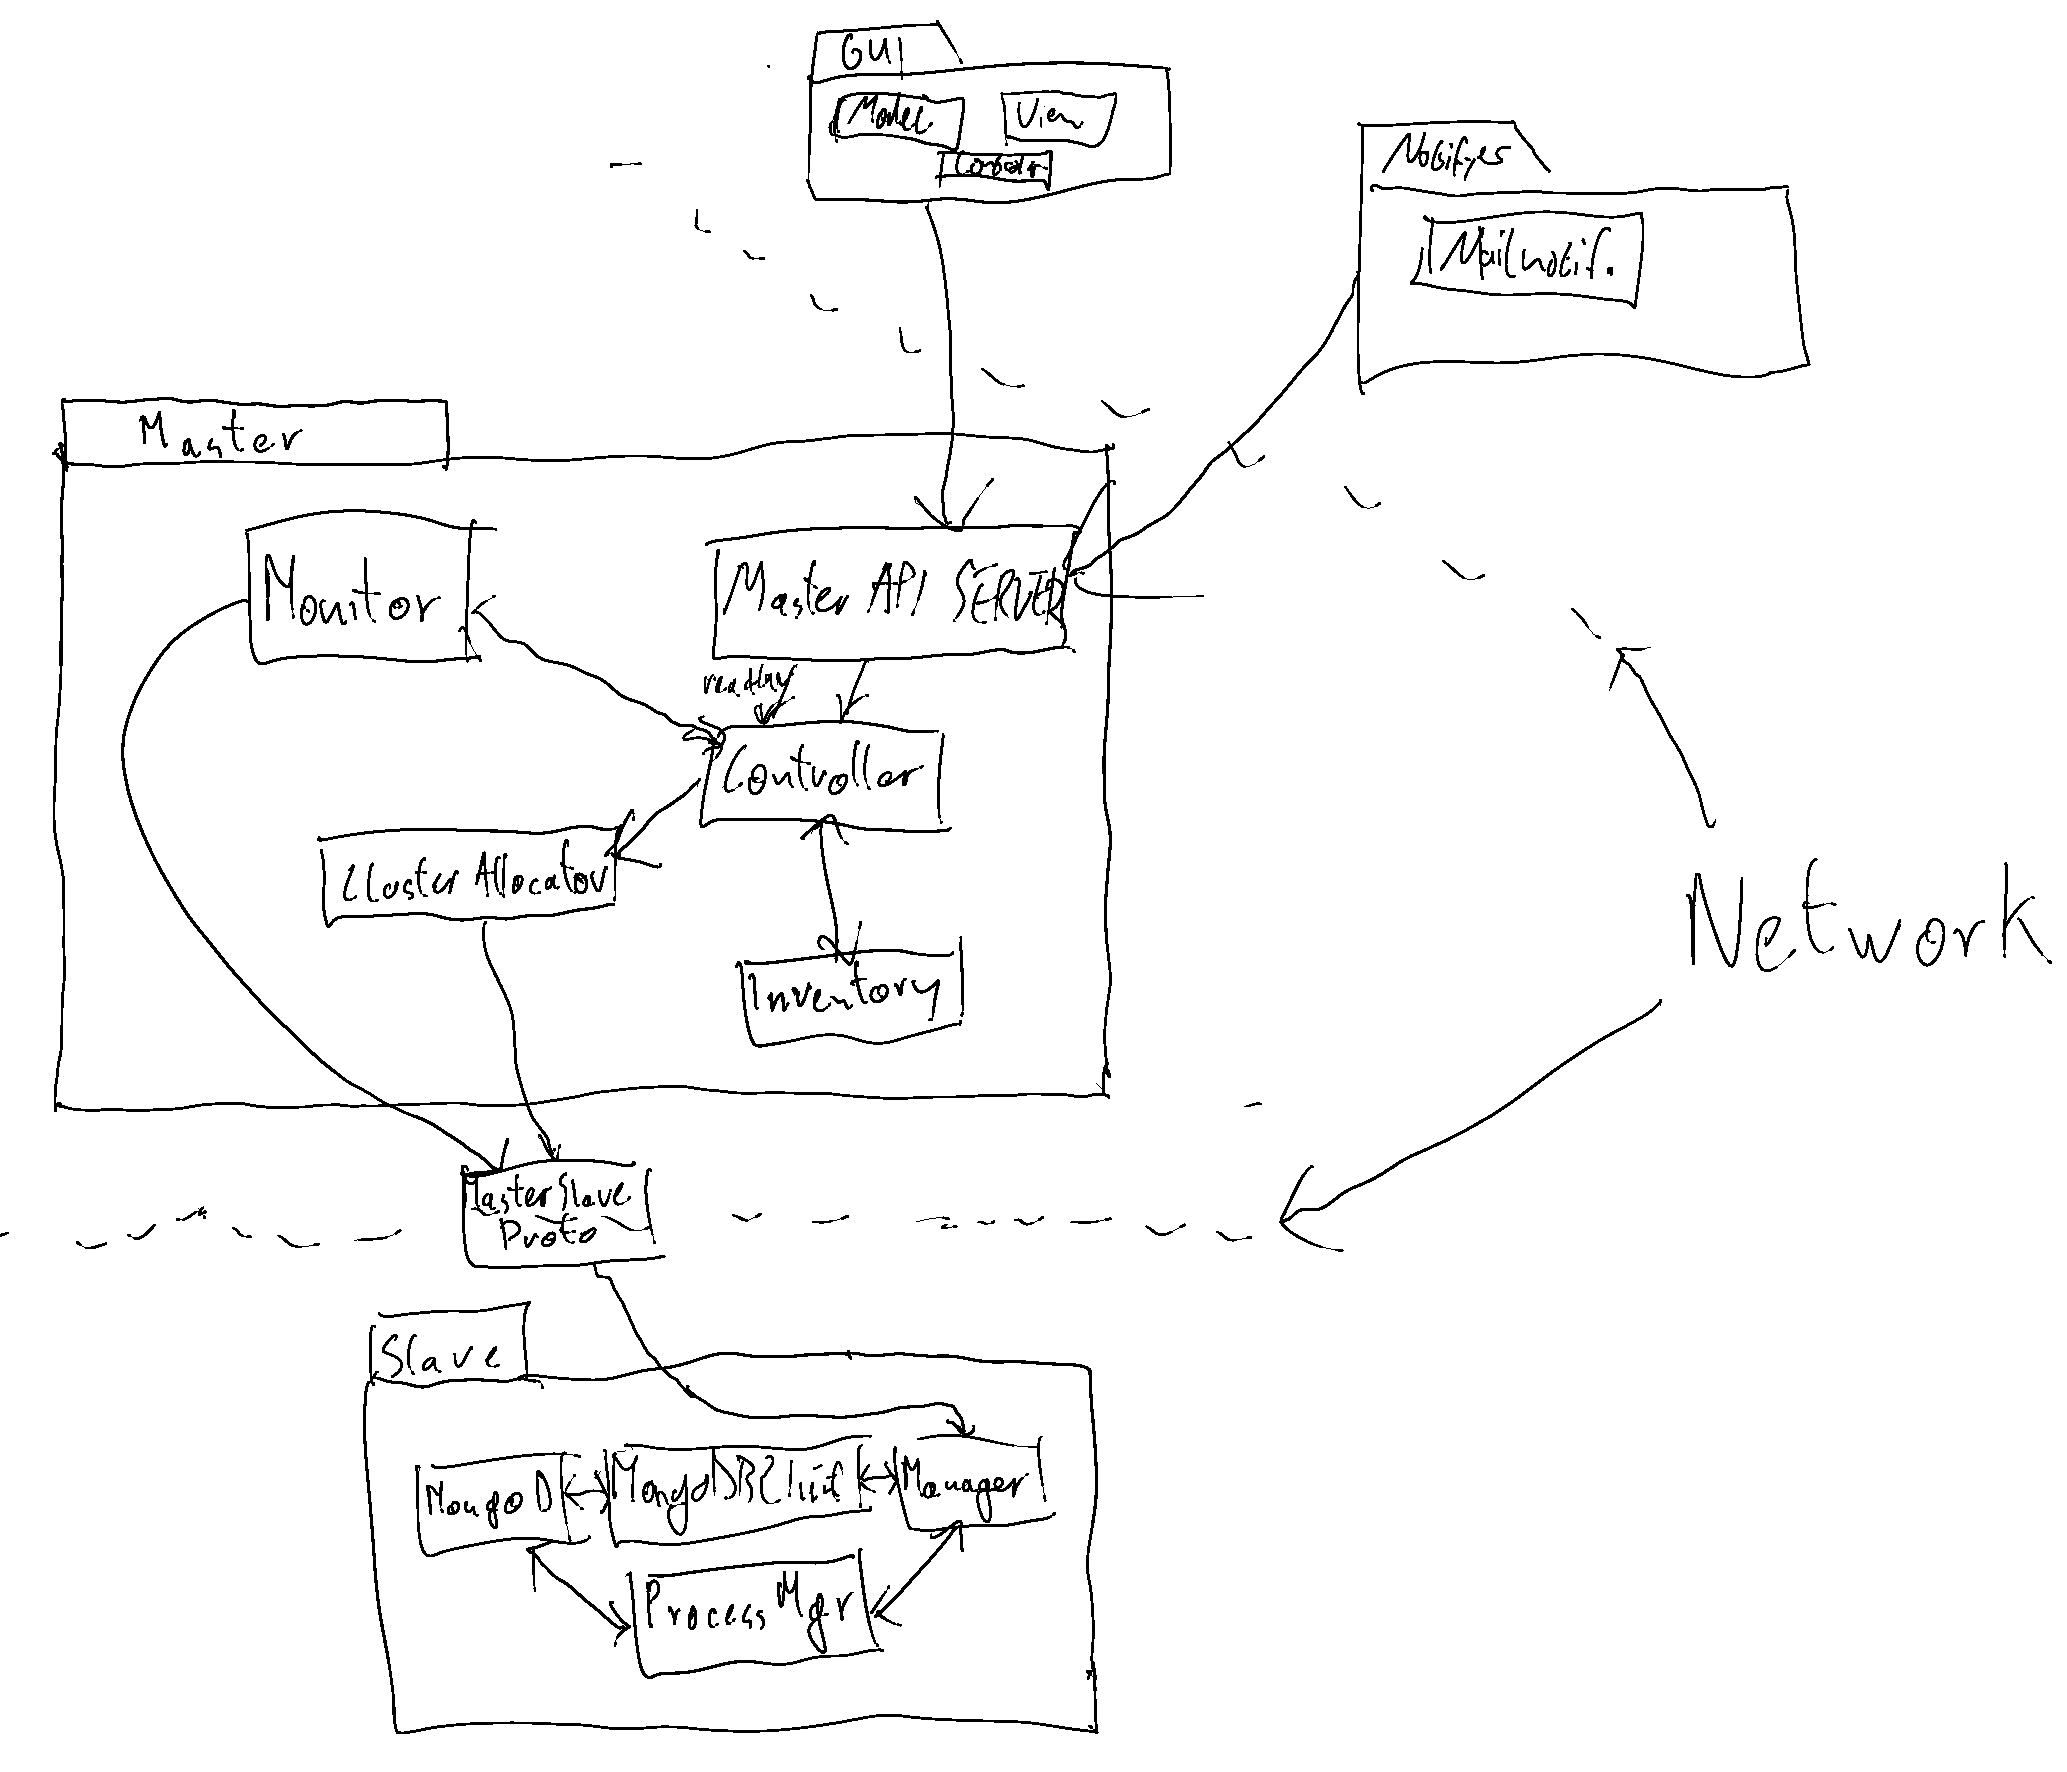
\includegraphics[width=\textwidth]{moduleplan}
\begin{description}
	\oitem{SM}{} Master::APIServer
	\oitem{SM}{} Master::Controller
	\oitem{SM}{} Master::Inventory
	\oitem{SM}{} Master::ClusterAllocator
	\oitem{SM}{} Master::Monitor
	\oitem{SM}{} MasterSlaveProtocol
	\oitem{SM}{} Slave::Controller
	\oitem{SM}{} Slave::MongoDBClient
	\oitem{SM}{} Slave::ProcessManager
	%Angular und so...
	\oitem{SM}{} GUI::Model
	\oitem{SM}{} GUI::View
	\oitem{SM}{} GUI::Controller
	\oitem{SM}{} NotificationManager::MailNotifier
	\oitem{SM}{} NotificationManager::APIClient
	\oitem{SM}{} NotificationManager::Controller
\end{description}
\section{Funktionale Anforderungen}
% Format: Substantiviertes Verb am Anfang („Bestimmen von X“, nicht „Bestimmung von X“, „Bestimme X“ oder „X bestimmen”).
\subsection{Kernfunktionen}
\begin{description}
\oitem{F}{testtest}
Test
\oitem{WF}{testestest}
test
\end{description}

\subsection{Vorberechnung}
\begin{description}
\oitem{F}{test}
test
\oitem{WF}{test}
test
\end{description}

\subsection{Benutzerschnittstelle}
\begin{description}
\oitem{F}{test}
test
\oitem{WF}{test}
test
\end{description}


\section{Nichtfunktionale Anforderungen und Qualitätsziele}

\begin{description}
\oitem{NF}{ntest} test
\end{description}

\section{Userinterface}
%Form:
%Name [: Beschreibung]
%Beschreibung: satz ohne subjekt, also klein und ohne Punkt; Strichpunkt getrennt
\subsection{Hauptfenster}

%\begin{enumerate}
%\item
%\end{enumerate}

%text...

\section{Globale Testfälle und Szenarien}
% Vorbedinung, Aktionen, Nachbedingung 
\subsection{Funktionssequenzen}
Bei allen Testfällen gilt als Vorbedingung, dass \mamid gestartet ist (außer es ist explizit gefordert, dass es gestoppt ist).
\begin{description}
\itemsep 1em
\subsubsection{Kernfunktionen}
\oitem{TF}{testen} a testcase.
\testfall[\ref{WK:beschlArc}] %testet:
    {foo} %vorbedingung
    {bar} % ablauf
    {jon} % erwa. ergebnis
\end{description}
\subsection{Testszenarien}
% all. vorbed.
\begin{description}
\oitem{TS}{test} blah
\begin{itemize}
\item ...
\end{itemize}
\end{description}

\subsection{Datenkonsistenzen}

\begin{description}
\oitem{TD}{blah} blah
\end{description}

\section{Entwicklungsumgebung}
\begin{description}
\item[Team communication] Slack
\item[Dokumentation] \LaTeX{}
\item[UML-Planungswerkzeug] UMLet
\item[IDE] ...
\item[Qualitätssicherung] ...
\item[Versionskontrolle] Git
\end{description}
\newpage
\glsaddallunused
\makeatletter
\newglossarystyle{myAltlist}{
  \glossarystyle{altlist} % base this style on altlist
  \renewcommand*{\glossaryentryfield}[5]{
  \item[\glsentryitem{##1}\glstarget{##1}{##2}]
    \mbox{}\par\nobreak\@afterheading
    ##3\glspostdescription\space On page ##5.
  }
}
\makeatother
\glsaddall
\printglossary[type=main, title={Glossary}, toctitle={Glossary}, style=myAltlist]

\end{document}
